\chapter{XBee}
\label{cha:XBee}

\section{ZigBee模块概述}

无线通信协议是在无线设备之间进行数据交换的一组规则。RF模块根据模块及其无线固件支持特定的无线通信协议。

以下是XBee无线模块支持的协议的完整列表:

\begin{itemize}
    \item IEEE 802.15.4
    \item ZigBee
    \item ZigBee Smart Energy
    \item DigiMesh (Digi proprietary)
    \item ZNet
    \item IEEE 802.11 (Wi-Fi)
    \item Point-to-multipoint (Digi proprietary)
    \item XSC (XStream-compatible)
\end{itemize}

\begin{figure}[htbp]
    \centering
    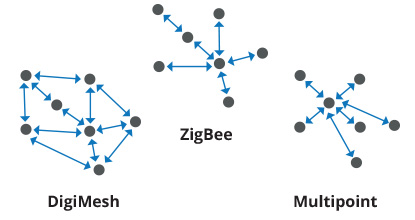
\includegraphics[width=0.5\columnwidth]{radio_comm_protocols.png}
    \caption{不同协议组网方式对比}
    \label{fig:radio_comm_protocols}
\end{figure}

并非所有XBee设备都可以运行所有列出的通信协议。XBee硬件和无线固件的组合决定了XBee设备可以执行的协议。

\section{固件升级}

本地设备设置AP=2 即 API mode 能使用Network Working Mode,以便升级固件。

用XBee 3 无线连接淘宝买的XBee Pro S2B需要先下载lagacy XBee Firmware。但不能直接无线更新固件,还是需要用USB连接到电脑上烧写新固件。XBee3则可以直接无线更新。

这就决定了小车上尽可能使用XBee3,虽然要比XBee S2B贵3-4倍。当然也可以直接在我们的PCB上画FT232接USB口以便更新固件使用,或者预留编程口直接使用编程线。

只有以下这些模块才能无线更新固件:

\begin{itemize}
    \item XBee/XBee PRO SX
    \item XLR Pro Module
    \item XBee/XBee PRO 802.15.4 (S2C module versions only)
    \item XBee/XBee-PRO DigiMesh 2.4 (S2C module versions only)
    \item XTend RF Module Family (SX module versions only)
    \item XBee/XBee-PRO ZB and Programmable XBee-PRO ZB
    \item XBee/XBee-PRO ZB SMT and Programmable XBee-PRO ZB SMT
    \item XBee-PRO 900HP and Programmable XBee-PRO 900HP
    \item XBee 865LP and Programmable XBee 865LP
    \item XBee3 (Zigbee, DigiMesh 2.4, and 802.15.4)
\end{itemize}

\section{AP参数}

XBee无线模块的操作模式建立了用户或连接到XBee的任何微控制器通过UART或串行接口与模块进行通信的方式。

取决于固件及其配置,无线模块可以在三种不同的操作模式下工作:

\begin{itemize}
    \item Application Transparent (AT) operating mode
    \item API operating mode
    \item API escaped operating mode
\end{itemize}

在某些情况下,无线模块的运行模式由固件版本(确定运行模式是AT还是API)以及固件的AP设置(确定API模式)决定。在其他情况下,操作模式仅由AP设置确定,该设置允许您将模式配置为AT(AP = 0),API(AP = 1)或API Escape(AP = 2)。

\subsection{AT}

在AT (Application Transparent) 透明操作模式下,无线模块接收的所有串行数据都排队等待RF传输。当模块接收到RF数据时,数据将通过串行接口发送出去。

要配置在AT中运行的XBee模块,必须将其置于命令模式下以发送配置命令。

当无线模块在AT工作模式下工作时,必须使用命令模式 command mode 界面来配置设置。

要进入AT命令模式,在一秒钟内发送三个字符的命令序列(通常为"+++")。一旦启动了AT命令模式,该模块将发送"OK \\ r",启动命令模式计时器,并且无线模块能够接收AT命令。

AT命令的结构为:

\begin{tcolorbox}
    AT[ASCII command][Space (optional)][Parameter (optional)][Carriage return]
\end{tcolorbox}

例如:

\begin{tcolorbox}
    ATNI MyDevice\textbackslash{}r
\end{tcolorbox}

如果在命令模式超时内未收到有效的AT命令,则无线模块将自动退出AT命令模式。您还可以通过发出CN命令来退出命令模式:

\begin{tcolorbox}
    (ATCN\textbackslash{}r)
\end{tcolorbox}

\subsection{API}

API(Application Programming Interface 应用程序编程接口)操作模式是AT模式的替代。API操作模式要求通过结构化接口与模块进行通信。换句话说,数据通过API框架进行通信。

API指定了如何使用串行接口从模块发送和接收命令,命令响应和模块状态消息。使用API​​操作模式,可以:

\begin{itemize}
    \item 配置XBee模块本身。
    \item 在网络中配置远程模块。
    \item 管理数据到多个目的地的传输。
    \item 接收每个发送的射频数据包的成功/失败状态。
    \item 标识每个接收到的数据包的源地址。
\end{itemize}

取决于AP参数值,无线模块可以以下两种模式之一运行:API(AP = 1)或API Escape(AP = 2)操作模式。

API转义操作模式(AP = 2)与API模式相似,不同之处在于,在API转义模式下工作时,必须转义API框架特定数据的某些字节。由于XCTU与API和API转义操作模式均兼容,因此您无需手动转义字符。

API转义操作模式通过防止与特殊字符(例如帧开始字节(0x7E))发生冲突,提高了RF传输的可靠性。API非转义(API = 1)操作仅依靠起始定界符和长度字节来区分API帧。另一方面,在API转义模式下,那些特殊字节被转义。由于0x7E只能出现在API数据包的开头,因此,如果在处于API转义模式下的任何时间接收到0x7E,则模块始终可以“假定”新数据包已经开始。

在以API转义模式发送或接收API帧时,必须对特定数据值进行转义(标记),以免干扰数据帧序列。

要转义数据字节,请插入0x7D,然后在其后跟要转义的字节与0x20进行XOR。需要转义的数据字节如下:

\begin{itemize}
    \item 0x7E: Frame delimiter
    \item 0x7D: Escape
    \item 0x11: XON
    \item 0x13: XOFF    
\end{itemize}

XCTU在与API转义的无线电模块进行交互时会自动转义适当的字符。

API帧是在无线电模块的串行接口上​​以API或API转义操作模式进行配置时发送和接收的结构化数据。API框架用于与模块或网络中的其他模块进行通信。API框架具有图~\ref{fig:api-frame}所示的结构:

开始符 Start delimeter 帧的第一个字节,由一个特殊的比特序列组成,这些比特序列指示数据帧的开始。它的值始终为0x7E。作用是检测新的输入帧。

长度 Length 指定帧数据字段中包含的字节总数。它的两个字节的值不包括起始符,长度和校验和。

帧数据 Frame data 由API标识符和特定于API标识符的数据组成。特定数据的内容取决于API标识符(也称为API帧类型)。

校验和 Checksum 帧的最后一个字节。它有助于测试数据的完整性,并通过获取其之前所有API帧字节(不包括前三个字节(开始符和长度))的哈希总和来计算。

\begin{figure}[htbp]
    \centering
    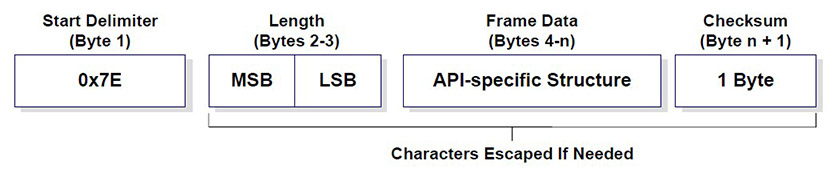
\includegraphics[width=\columnwidth]{concpts_api_frame_explained_80.jpg}
    \caption{API帧}
    \label{fig:api-frame}
\end{figure}


\section{XCTU的配置}

coordinator是中心节点,Router是小机器人的,他们的配置要注意,比如AP=2,DH/DL是地址,都设为零,因为按照api里定义的地址发送,配置里的目的地址就填零就行。配置如表~\ref{tab:XCTU}所示。

% Please add the following required packages to your document preamble:
% \usepackage{booktabs}
\begin{table}[htbp]
    \centering
    \begin{tabular}{@{}lll@{}}
    \toprule
             & Coordinator & Router \\ \midrule
    ID(相同即可) & 1234        & 1234   \\
    SC       & 8           & 8      \\
    ZS       & 2           & 2      \\
    JV       & 无           & 1      \\
    DH       & 0           & 0      \\
    DL       & 0           & 0      \\
    AP       & 2           & 2      \\ \bottomrule
    \end{tabular}
    \caption{XCTU配置}
    \label{tab:XCTU}
\end{table}